\documentclass[11pt,a4paper]{article}

\usepackage{fancyhdr}
\usepackage{parskip}
\usepackage[usenames,dvipsnames]{color}
\usepackage[colorlinks=true, linkcolor=BrickRed, citecolor=Blue, urlcolor=Blue, filecolor=Blue]{hyperref}
\usepackage{graphicx}
\usepackage{xcolor}
\usepackage{amssymb, amsmath}
\pagestyle{fancy}

\newcommand{\mail}[1]{\href{mailto:#1}{#1}}

\begin{document}

\thispagestyle{fancy}

%Include the logo in this code when it is finished
\centerline{\textbf{GAMBIT: Global And Modular BSM Inference Tool}}



\centerline{\textbf{Code Policies}}\bigskip 

\section{Coding Style}

\subsection{Guidelines (rules)}

\subsubsection{File naming} All file extensions to be .hpp (headers) and .cpp (source).

\subsubsection{Code structure naming conventions} The only things to be called \begin{verbatim}<blah>Bit\end{verbatim} are the physics modules (ColliderBit, DarkBit, FlavBit, etc) and the scanner module (ScannerBit). No sub-categories of code within these is a `Bit', nor are any of the Utils, Core, Logs, Models, etc. The general rule is that Bits are things that can and will be released and able to function on their own with the addition of a simple driver program.

\subsubsection{Namespaces} 
\begin{itemize}
  \item Everything goes in \begin{verbatim}Gambit\end{verbatim} namespace
  \item backend objects go in \begin{verbatim}Gambit::Backend\end{verbatim}
  \item module functions in \begin{verbatim}Gambit::<module_name>\end{verbatim}
  \item No virus-like global ``using namespace blah'' is allowed in headers; scoped use of namespaces only please.
\end{itemize}

\subsubsection{Header inclusion ordering} 
\begin{enumerate}
  \item C/C++ standard headers
  \item GAMBIT headers
  \item Boost headers
  \item Other required or contributed headers (e.g. yaml-cpp)
\end{enumerate}
This helps ensure that the GAMBIT overwrites of some of the Boost headers get applied universally (in the cases where they are actually invoked).

\subsubsection{Whitespaces} 
\begin{itemize} 
  \item No explicit TABs in files (spaces only)
  \item Does not have to be the same in each file, but keep it consistent within each file
\end{itemize}

\subsubsection{Variable names} No precise rule on naming, just keep your convention consistent within each file.

\subsubsection{Comments}
\label{comments} 
\begin{itemize} 
  \item keep them aligned and easy to read
  \item Each file to begin with a standard documentation comment header (found in the same folder as the source code for this document, or at \href{https://gambit.hepforge.org/trac/browser/Collaboration\%20Docs/Code\_Policies/standard_preamble.cpp}{https://gambit.hepforge.org/trac/browser/Collaboration Docs/\\Code\_Policies/standard\_preamble.cpp}).
\end{itemize} 


\subsection{Recommendations (not rules)}

Align your braces vertically, i.e. 
\begin{verbatim}
do this
{ 
  my.awesome.code = this;
}

not this {
  my.lousy.code = this; }

nor this {
  my.lousy.code = this; 
}
\end{verbatim}

\section{Target Compilers}

\begin{itemize}
\item[]\textbf{icc}/\textbf{ifort} v12.1.0 and later
\item[]\textbf{gcc}/\textbf{gfortran} v4.4.7 and later
\item[]\textbf{clang}/\textbf{fort equivalent?} first (upcoming) version to support openMP
\end{itemize}

\subsection{Library requirements/compatibilities}

\begin{itemize}
\item[]\textbf{Boost} v1.41 and later
\end{itemize}

Maybe make yaml-cpp and HepMC required libs rather than contributed libs at some point too.

\subsection{Build system}

GNU autotools to start with.  Probably cmake later.

\section{Hosting}

Hosting is on HEPForge, who have kindly implemented git as an alternative to svn just for us.

\section{Documentation}

Doxygen.  All code needs at the very least to come with an email address, detailing who to abuse when the code breaks and needs to be fixed but cannot due to lack of comments.  A less painful alternative, \textbf{very} strongly encouraged, would be to actually document your code properly in the first place.  There is a standard-issue GAMBIT comment/documentation preamble available; see Sec.~\ref{comments}.

\section{Bug Tracking}

Extensive logging and error tracking is implemented in the GAMBIT core now.  Bug tracking should be carried out with the TRAC ticketing system on the Wiki.

\section{Structure}

\textbf{PS, Apr 2014:} This is a bit of a peek into GAMBIT past, at the time the whole thing was conceived.  Some aspects remain accurate today, some don't.

\textbf{PS, Oct 2012:} The following is a first rough attempt to explain some details of the code structure we envisioned at the first meeting.  I'm sure there is probably a better way to explain this, with fancy diagrams and so on, but exactly what that method is didn't yield itself to a half hr of Googling (unless we want to go for full-blown UML diagrams, which seems pretty involved).  Some of this stuff is already implemented in SUFit, some not.

We refer to the different main bits of the code as `modules', with the `core' module (CoreBit) controlling all inter-module communication.  The code will consist of the core, a series of `physics modules' (HEColliderBit, LEColliderBit, DarkTheoryBit, RelicBit, DirectBit, IndirectBit, maybe later some more like NeutrinoBit, CosmoBit, etc), the scanner module (ScannerBit) and the model module (ModelBit).  The scanner module takes care of selecting the scanning algorithm and running it.  The model module defines the actual theory, model parameterisation and spectrum calculation, including full specification of how any nuisance parameters enter (e.g. dark matter halo modelling).  The physics modules provide calculations of observables and likelihoods.  Experimental data is carried within the physics modules, and associated internally in the physics modules with likelihood functions, in whatever way the individual module authors see fit.  The physics modules should be able to operate as standalone packages, and will be released as such.  The scanner module might be useful as a standalone package too.  The general modularisation strategy is that the core handles all administration, the physics modules all physics and likelihood calculations, the model module all model-dependent definitions, and the scanner module all scanning and statistical issues.  Plotting and statistical analysis of samples after a scan is complete will be handled by an additional external package; we can ship one or more such packages as part of GAMBIT (Pippi being one obvious choice).

Physics modules will provide (up to) two types of functions accessible by the core: observable calculators, and likelihood calculators.  Users may write their own additional observable or likelihood calculator function and add it to a physics module, or may add an entire new module.  New modules might add new observables or likelihoods, or just preferred versions of existing ones.  Data need never be explicitly revealed to the core by the physics modules per se, but should be simply associated internally with likelihood functions.  In principle `observable' functions can return anything, including raw experimental data, but this is not envisaged as the typical mode of operation.  Likelihood functions in physics modules may be explicitly implemented within the module, or may simply point to common likelihood functions defined in a separate utilities module (UtilsBit?).  UtilsBit will need to ship with every standalone physics module.  Observable functions in physics modules may also be explicitly implemented within the module, or may call a routine from another external code in order to obtain the value of the observable for the parameter values in question.

\begin{figure}[tbp]
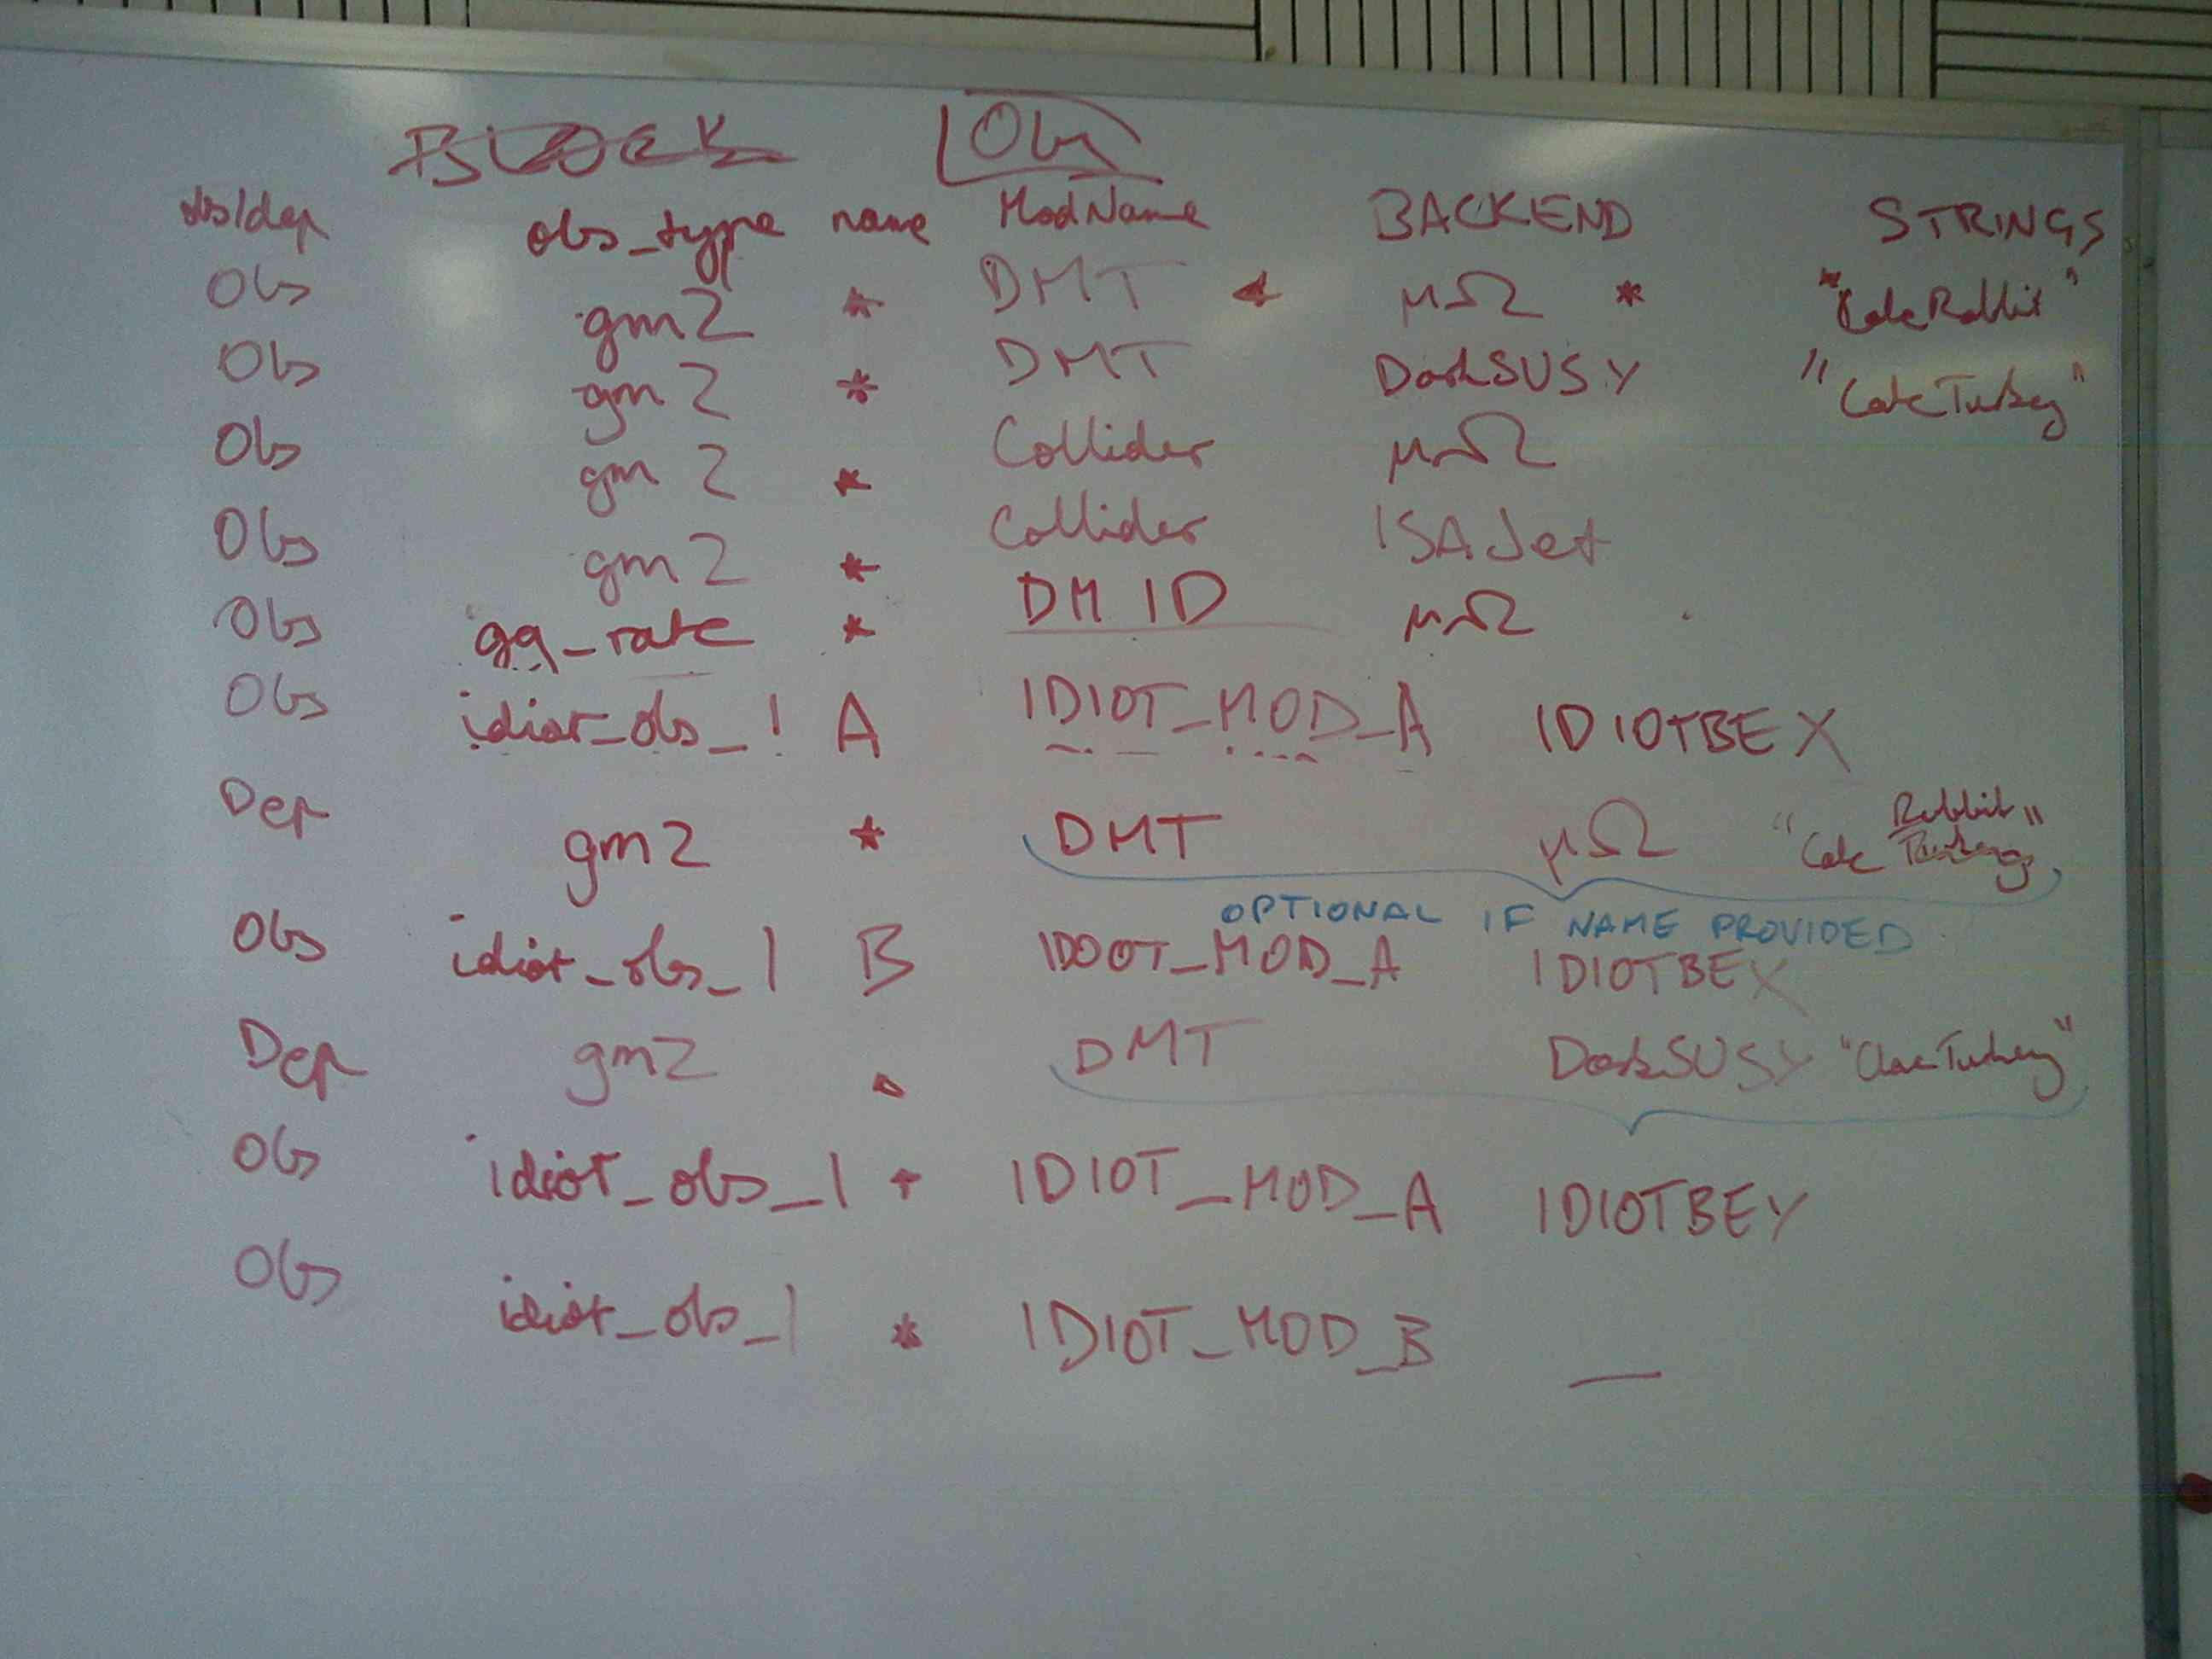
\includegraphics[width = 0.8\linewidth]{Code_Policies/fig1}\\
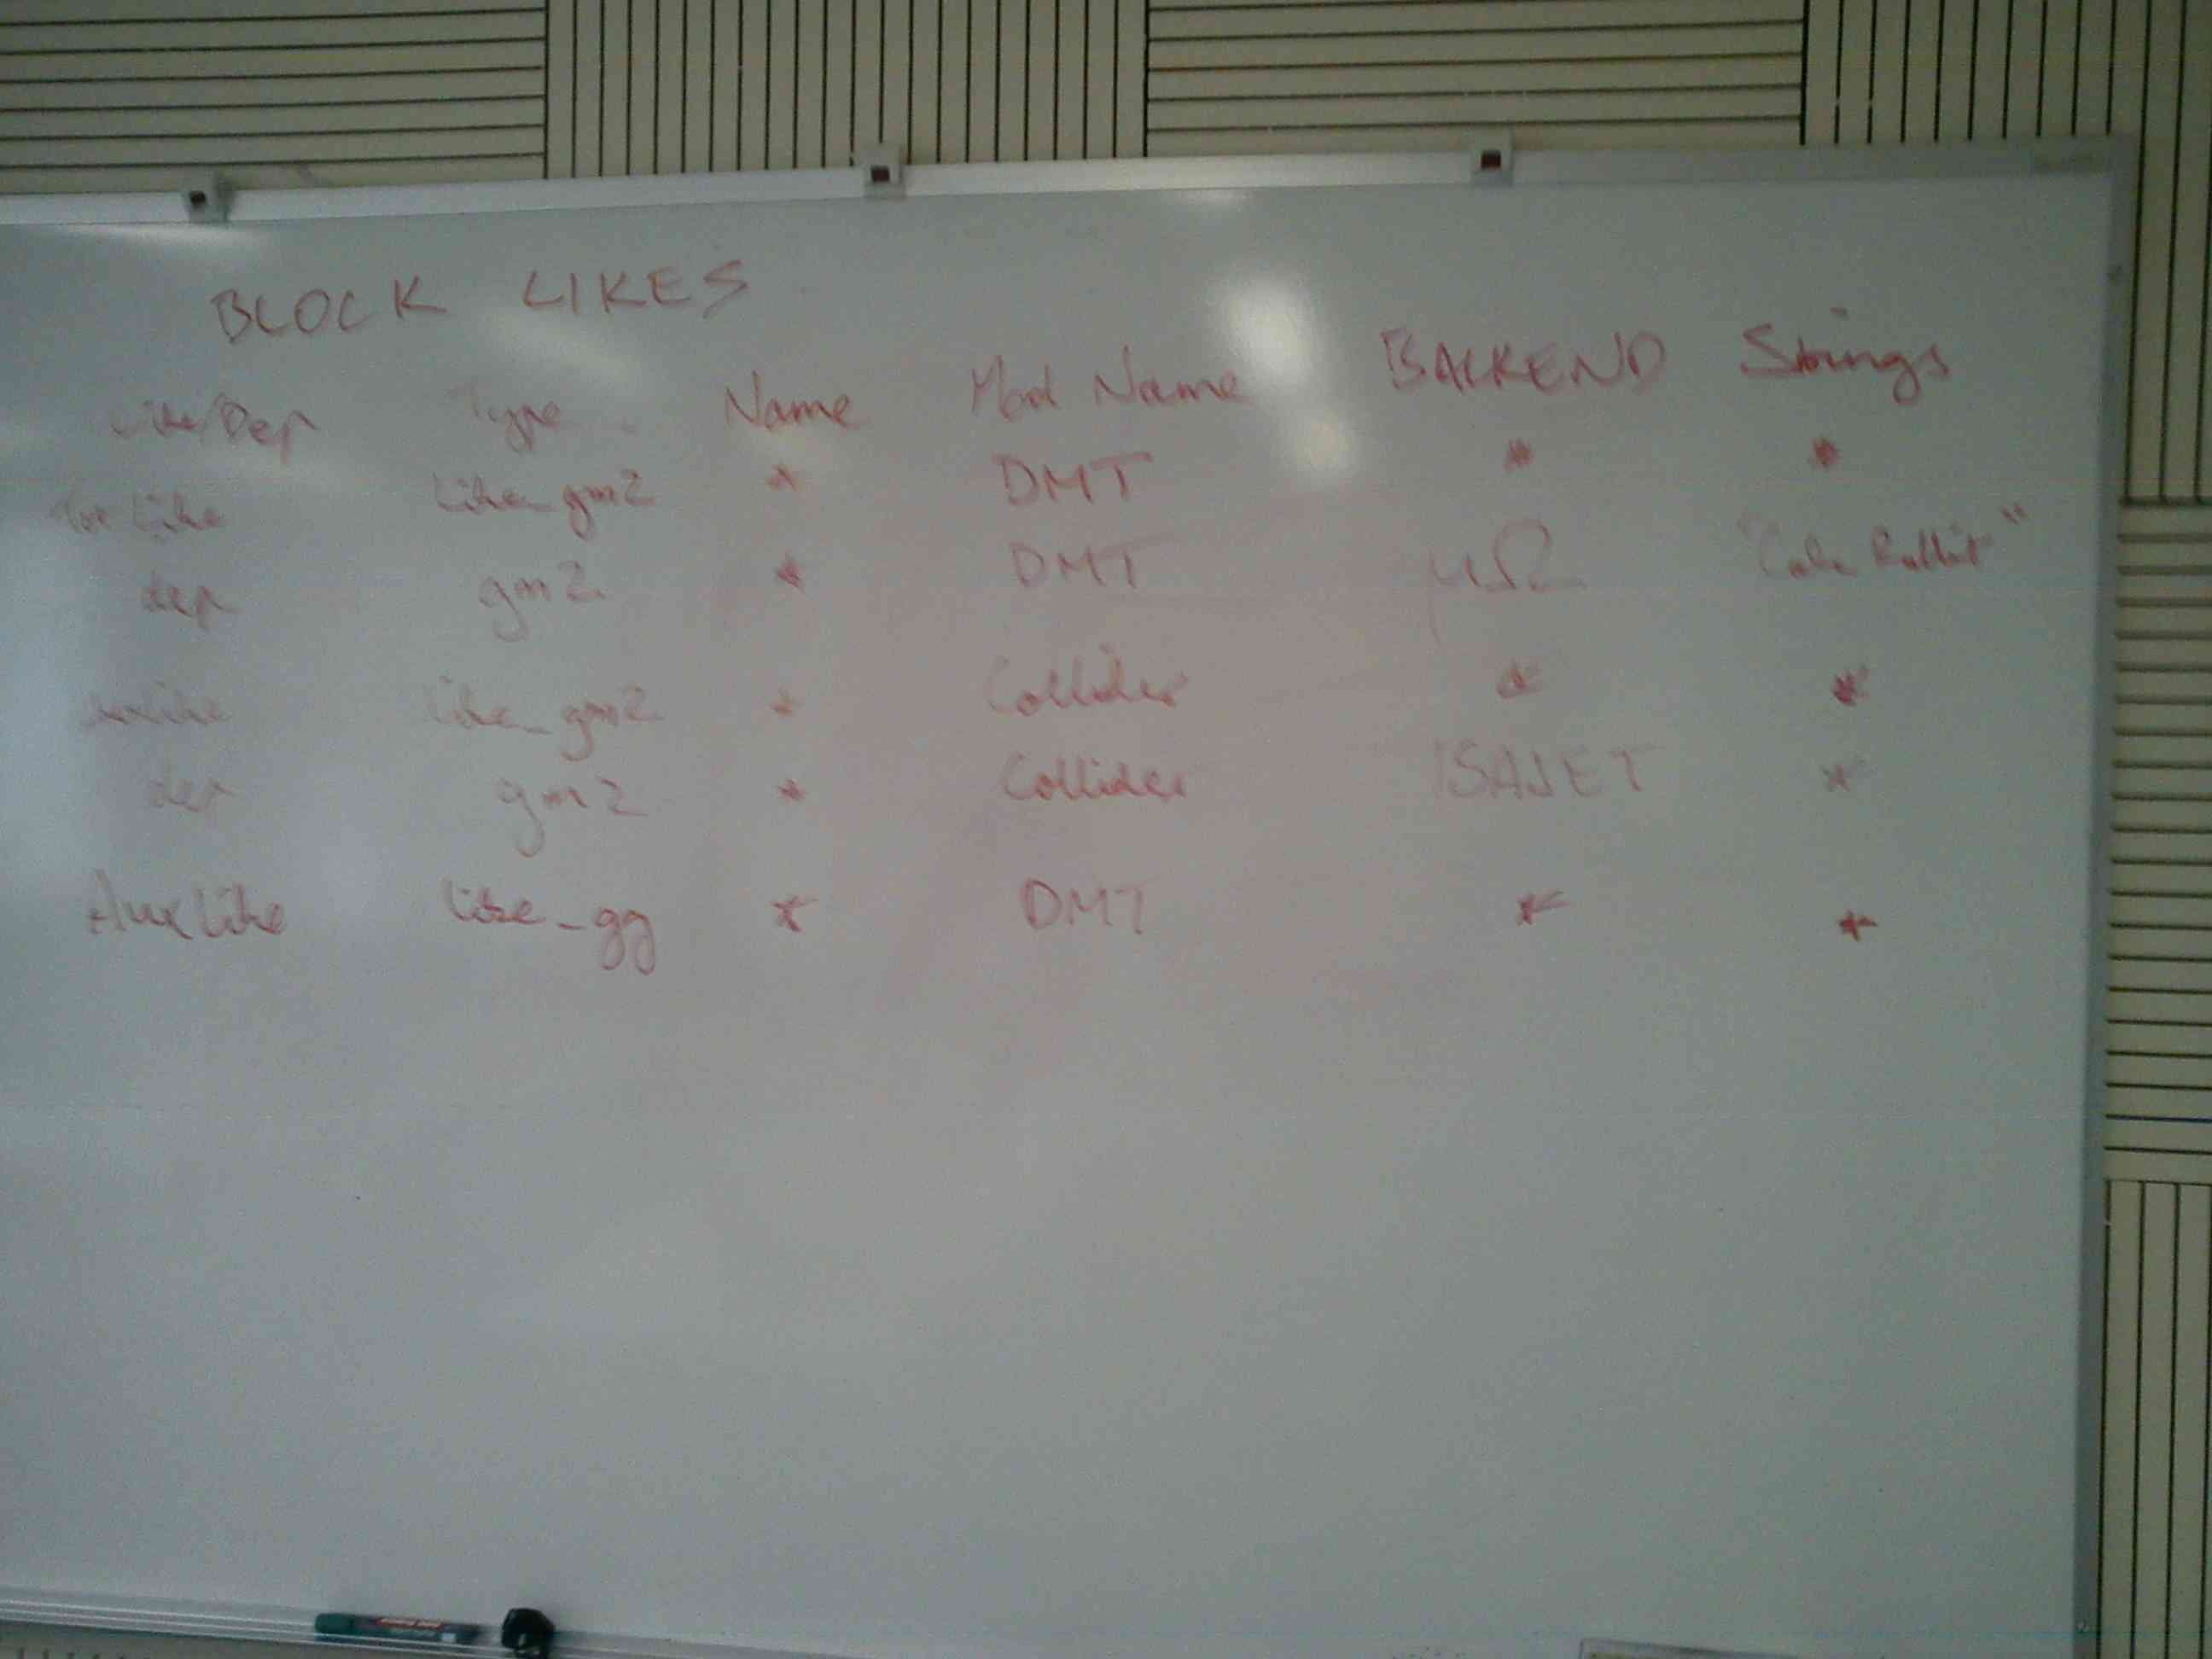
\includegraphics[width = 0.8\linewidth]{Code_Policies/fig2}\\
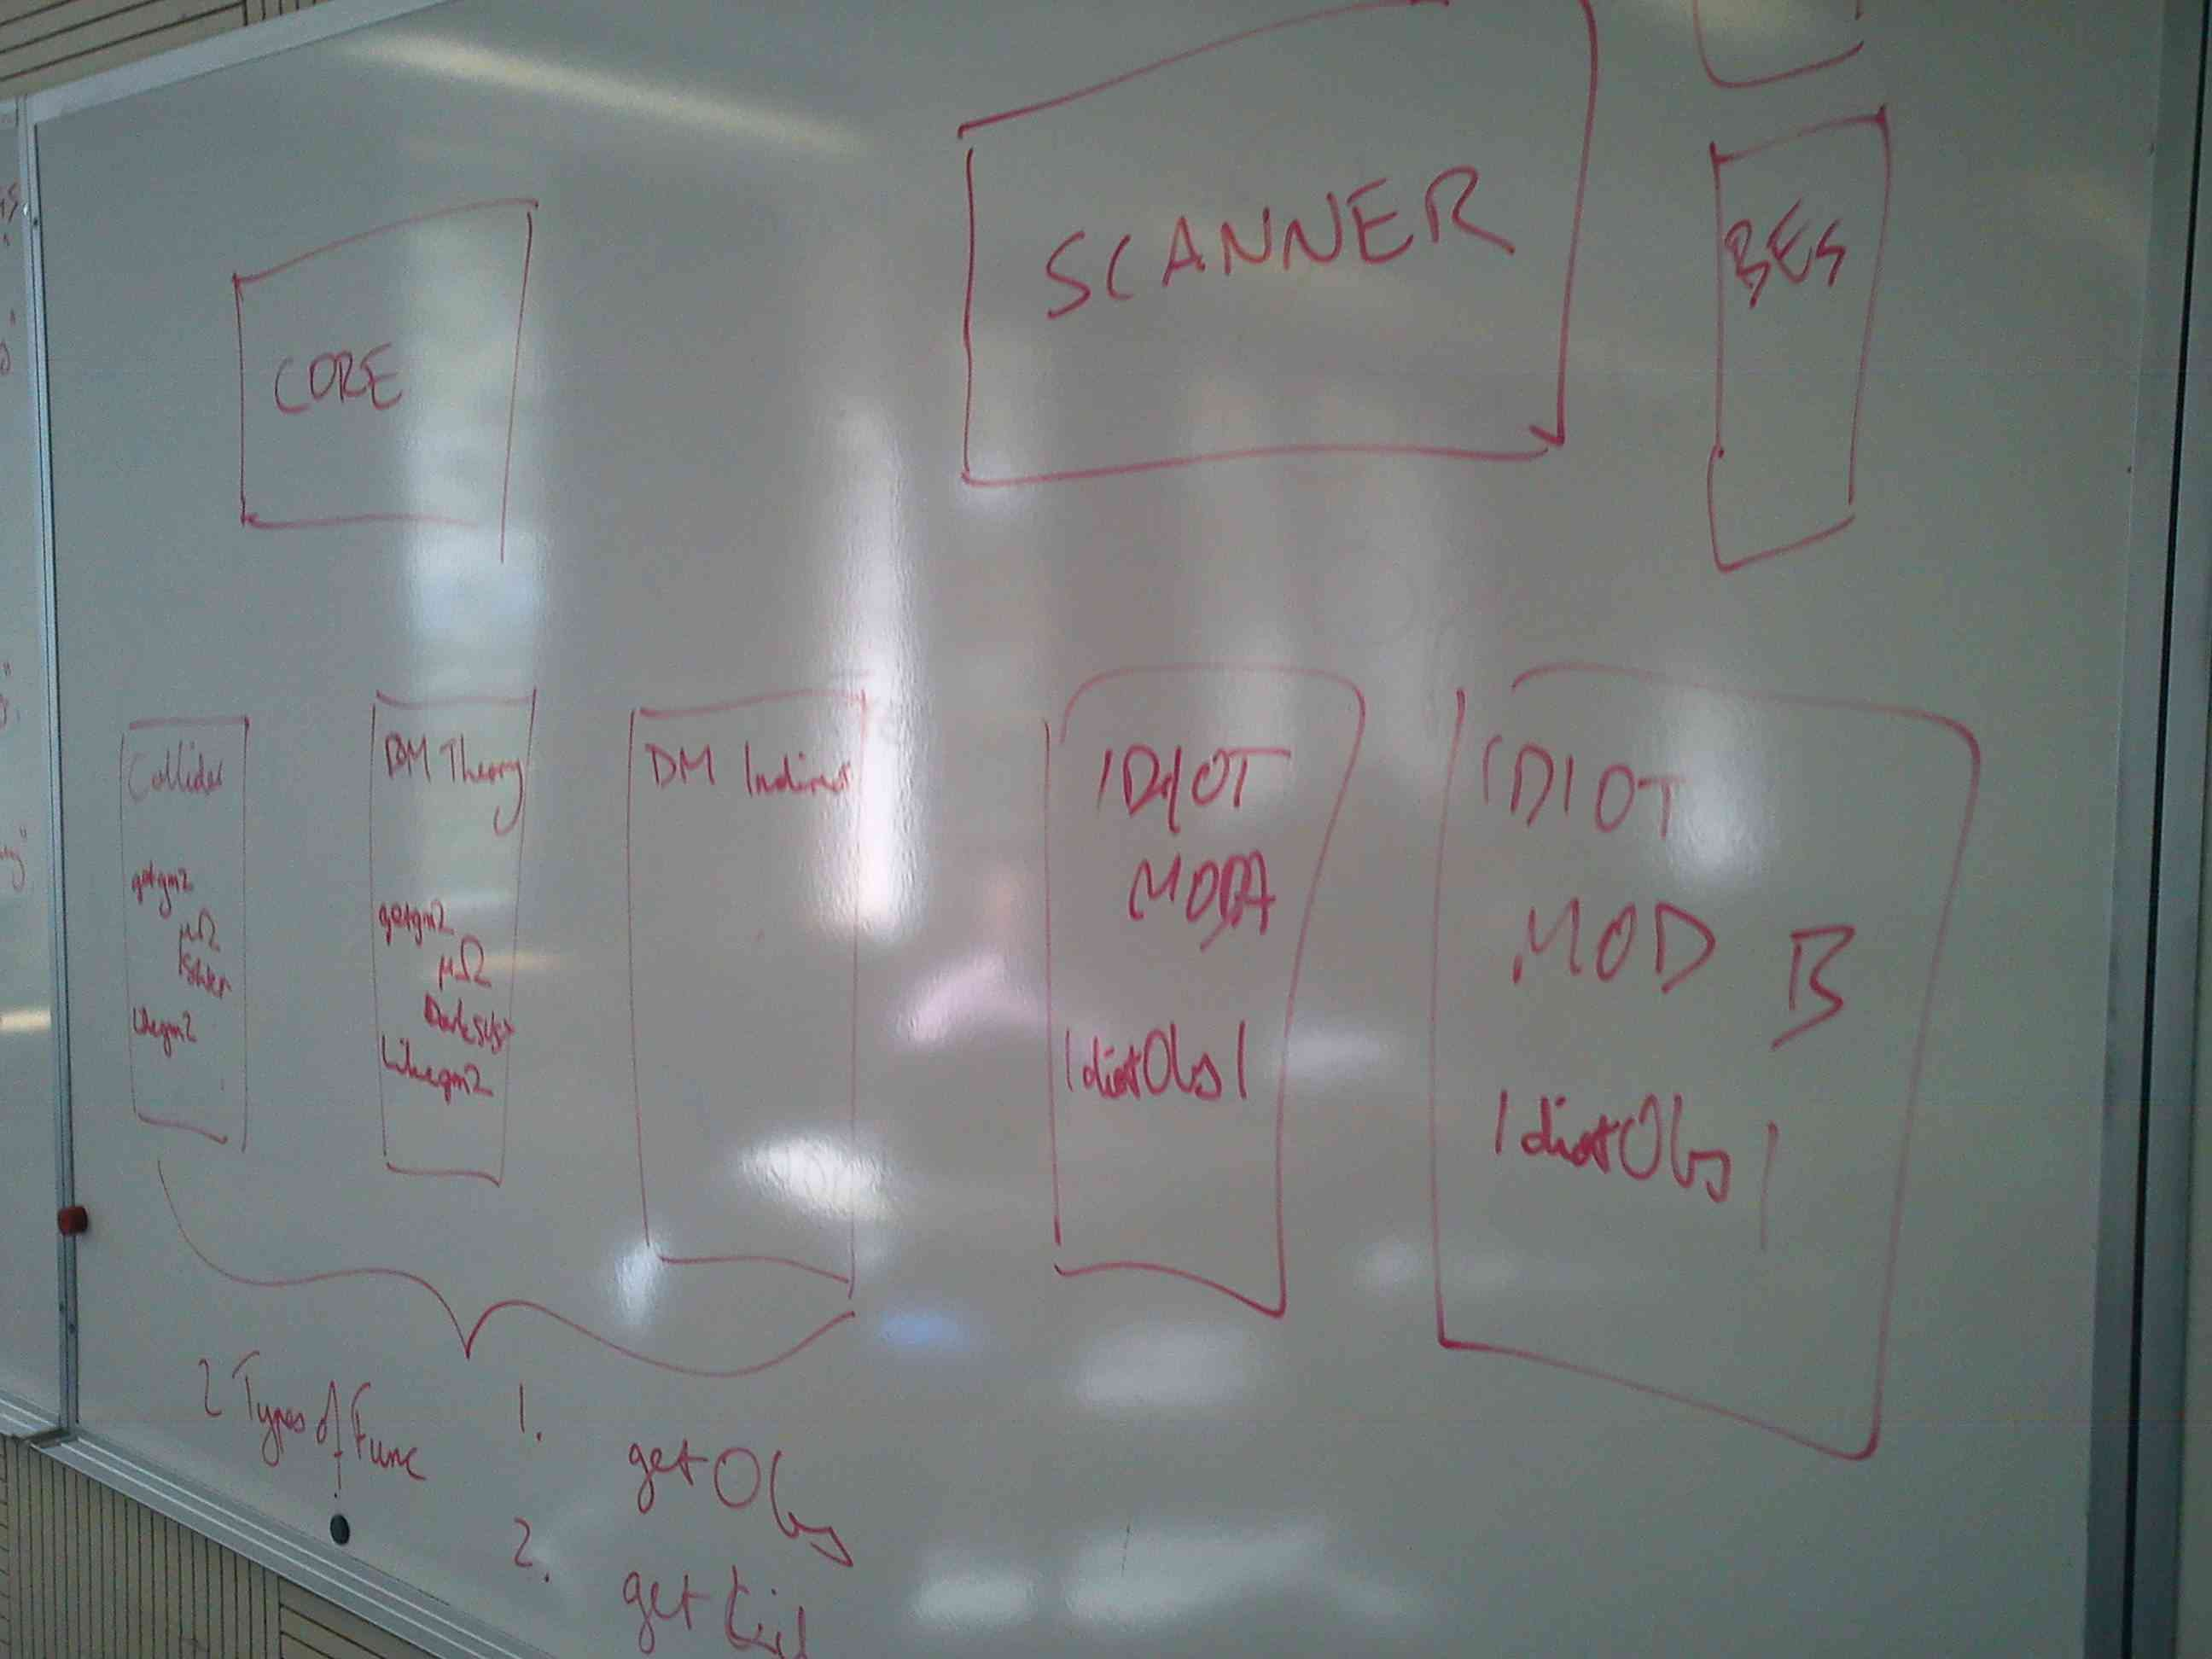
\includegraphics[width = 0.8\linewidth]{Code_Policies/fig3}
\caption{Example input ASCII file formats for OBS (top) and LIKE (middle) blocks, as well as a very rough schematic outline of GAMBIT code structure (bottom).  Crappy wobbly camerawork by Pat.}
\label{figure1}
\end{figure}


To set up a scan, the core will construct a likelihood container object (the class definition of which would probably be part of CoreBit), containing pointers to all the observable and likelihood functions to be called for a given scan (as specified in an input ACSII file).  The core will pass this object to the scanner module (more concretely, it would pass a pointer to the likelihood container object to the constructor of a scanner object).  The scanner(or the likelihood container object itself) will then call each of the likelihood functions contained in the likelihood container object in turn, for each point in the scan.

As each member function of the physics modules is called, the likelihood container object will place the resulting observables and likelihoods into some sort of dictionary structure (like a Python dictionary -- we are hoping Hugh can implement a really nice C++ emulation of a Python dict, or knows something already in existence).  Observable and likelihood functions requiring inputs will be provided these by reading the relevant key-value pair from the dictionary.  The model definition provided by ModelBit will define a ModelParameters object, containing the values of the model parameters at a given point in parameter space; this will also be held in the dictionary.  After the evaluation of all observable and likelihood functions for a given point, the contents of the dictionary will be written to disk (as the next point in the output `chain').

Every observable and likelihood function will have an associated set of tags, indicating what type of observable/likelihood it provides, and what type of observable(s) it requires as input.  The core will parse these tags at the beginning of a scan, and ensure a calling order that takes all the necessary dependencies of different observable and likelihood function calls into account.  Similarly, each function will have a TypicalExecutionTime tag, which will be used to call the fastest functions first, so that slower computations can be skipped if a point exhibits a sufficiently low likelihood already from the fastest likelihood calculations.

Observables and likelihoods to be calculated and/or used in a scan, as well as specifics of any dependencies that cannot be automatically resolved by the core, will be specified in the input ASCII file as outlined in Fig.~\ref{figure1}.  Here some rather nasty examples of multiple calculations of a single observable a number of different ways are given, showing how the dependency functionality might be used.  The `name' field is present to allow two copies of an otherwise identical observable calculation to be carried out with two different versions of a dependent observable.  Asterisks are used to indicate that a field is to be `automagically' filled in by the core.  The core would throw an error if the values of these fields are not able to be automatically uniquely determined (ignore asterisks in ModName and BackEnd entries in top row of observable example).

This example also shows how different likelihoods may be calculated and either included in the actual total scan likelihood (TotLike in first column), or just calculated and output in final chains without being included in the overall joint likelihood (AuxLike).  Every individual component of the total scan likelihood will automatically be output in final chains; observables will be included in the final chains only if they are explicitly indicated in the input file.  If a likelihood is specified that depends on a certain observable \textit{not} included in the input file explicitly as an observable, then the core will automatically identify the dependency and calculate the observable, provide it to that likelihood function and output the value of the likelihood function at each parameter combination to the chain, but \textit{not} include the value of the observable in the final output chain.

The ASCII input file will also be used to specify initialisation settings for the different modules, with a dictionary of settings generated from the input file passed to the constructor of each physics module object constructor, as well as the scanner object constructor.

External codes will be interfaced with via a common object class for each specific code, referred to as a BackEnd object (part of the UtilsBit module).  Physics modules may draw upon the same instance of a particular backend class (e.g. RelicBit and IndirectBit would probably want to use the same DarkSUSYBackEnd object), or may each create their own instances of such a class (e.g. HEColliderBit and LEColliderBit would need different PythiaBackEnd objects, as they would probably require different initialisation choices to be passed to Pythia; HEColliderBit might even require two different instances of PythiaBackEnd just on its own, one each for LHC and ILC work).  BackEnds will also carry flags corresponding to their capabilities; the functions they provide will indicate what unique physical observable quantity each function provides, and which known models it can be invoked for.  Physics module observable and likelihood functions will also need to carry tags indicating which models they are callable for (for observables, many of these will just be automatically inherited from the chosen BackEnd member functions; for likelihoods, in many cases model tags will not be required, as the the likelihood form will be model-independent).

ModelBit will also make use of the BackEnd class, in order to interface with spectrum generators.  At a later stage of code development (ie after the first physics paper), model specifications created with ModelBit will also implement Lagrangian and/or Feynman rules specifications, and interface with automatic cross-section calculators such as MadGraph via a BackEnd object.  The results of such cross-section calculations will either be somehow `deposited' into other backended external codes (likely a bit messy) or passed into the core for run-time reference by physics modules and (via the physics modules) other BackEnds.  Exactly how to set this up remains to be determined.

The model and scanner `modules' will essentially just be abstract model and scanner object base classes; the physics modules will each be specific daughter classes of an abstract PhysicsModule base class.  The inclusion of observable and likelihood functions into the specific daughter classes of PhysicsModule should also be (somehow) achieved as modularly as possible, with a view to making it possible to include new data and/or observables by adding a single source file rather than modifying existing code.  Adding new physics modules, scanners, models or backend codes should be a matter of writing only a new source file defining a new daughter class of the PhysicsModule, Scanner, Model or BackEnd abstract base classes.  With a bit of thinking, we can hopefully even make it possible to register and load these new libraries dynamically, without recompiling the rest of the GAMBIT code at all.

\end{document}
